\documentclass[pdftex]{beamer}

% Setup beamer look theme
\mode<presentation>
{
	\useinnertheme{rectangles}
	\useoutertheme{infolines}
	\usecolortheme{crane}
	\setbeamertemplate{navigation symbols}{}
}

% Use nicer font
\usepackage{palatino}
\usepackage{palatino,graphics,array,slashbox}

% Setup UTF-8 encoding
\usepackage[utf8]{inputenc}
\usepackage[T1]{fontenc}

% Setup czech language
\usepackage[czech]{babel}

% Include usefull packages
\usepackage{graphics}

% Include hyperlinks support
\usepackage{hyperref}
\hypersetup{colorlinks=true,linkcolor=black,urlcolor=black,unicode=true}

% Add support for simple URLs
\usepackage{url}

% Commands for CC license
\newcommand{\CcLongnameByNcSa}{\href{http://creativecommons.org/licenses/by-nc-sa/3.0/cz/}{Attribution-Noncommercial-ShareAlike}}
\newcommand{\CcImageBy}[1]{
\includegraphics[scale=#1]{../commons/graphics/cc-by-white.pdf}}
\newcommand{\CcImageNc}[1]{
\includegraphics[scale=#1]{../commons/graphics/cc-nc-white.pdf}}
\newcommand{\CcImageSa}[1]{
\includegraphics[scale=#1]{../commons/graphics/cc-sa-white.pdf}}
\newcommand{\CcGroupByNcSa}[2]{\CcImageBy{#1}\hspace*{#2}\CcImageNc{#1}\hspace*{#2}\CcImageSa{#1}}


\title{Úvod do jazyka C}
\subtitle{Cvičení - týden I}
\author[]{Mgr.~Šimon~Tóth}
\institute[FI@MU]{Fakulta informatiky @ Masarykova Univerzita}
\date{\today}

\newcommand{\CcNote}[1]{% longname
        Licencováno pod: \textit{Creative Commons #1 3.0 License}.%
}

\begin{document}
	\begin{frame}
		\titlepage
		\vfill
		\begin{center}
			\CcGroupByNcSa{0.33}{0.95ex}\\
			{\tiny\CcNote{\CcLongnameByNcSa}}
			\vspace*{2ex}
		\end{center}
	\end{frame}

\section{Organizační info}
\subsection{Úvodní test}

\begin{frame}
	\frametitle{Úvodní test}
	\begin{itemize}
		\item{\texttt{Student -> Odpovědníky}}
	\end{itemize}
\end{frame}

\subsection{Odevzdávání příkladů}

\begin{frame}
	\frametitle{Odevzdávání příkladů}
	\begin{itemize}
		\item{plně automatický systém}
		\item{odevzdávání nanečisto a naostro}
		\item{15..20 min. zpoždění mezi odevzdáním a opravou}
		\item{zdrojové kódy letos v SVN repozitáři}
	\end{itemize}
\end{frame}

\begin{frame}
	\frametitle{Oprava příkladu}
	\begin{itemize}
		\item{probíhá na serveru aisa}
		\item{gcc verze 4.5.1}
		\item{očekává přesnou strukturu v SVN}
		\item{pozor na velká / malá písmena}
	\end{itemize}
\end{frame}

\begin{frame}
	\frametitle{Email s opravou}
	\begin{itemize}
		\item{jako výsledek opravy dorazí email}
		\item{výstupy jsou záměrně mlhavé (chyby musíte hledat)}
		\item{případné dotazy raději na autora zadaní/testu}
		\item{technické problémy řeším já}
	\end{itemize}
\end{frame}


\section{Teorie}
\subsection{GCC}

\begin{frame}
	\frametitle{Překlad programu}
	\begin{enumerate}
		\item{ujistěte se zda máte správnou verzi gcc (4.5.1 na aise)}
		\begin{itemize}
			\item{\texttt{gcc --version}}
		\end{itemize}
		\item{zvolte správnou sadu přepínačů}
		\begin{itemize}
			\item{\alert{povinné:} \texttt{-std=c99 -pedantic -Wall}}
			\item{\alert{doporučené:} \texttt{-Wextra -Wwrite-strings -Werror}}
			\item{pro debugování: \texttt{-ggdb3}}
			\item{pro rychlý běh: \texttt{-O3 -strip -fomit-frame-pointer}}
		\end{itemize}
	\end{enumerate}
\end{frame}

\subsection{Fáze překladu}

\begin{frame}
	\frametitle{Postup překladu}
	Bylo na první přednášce.
	\begin{enumerate}
		\item{preprocessor}
		\item{převod do assembleru}
		\item{kompilace}
		\item{linkování}
	\end{enumerate}
\end{frame}

\subsection{Probráno na přednášce}

\begin{frame}
	\frametitle{Datové typy}
	\begin{itemize}
		\item{pozor na datové objemy}
		\item{standard garantuje}
		\begin{itemize}
			\item{minimální rozsahy}
			\item{základní vztahy}
		\end{itemize}
		\item{pozor na \texttt{sizeof(char)}}
	\end{itemize}
\end{frame}

\begin{frame}
	\frametitle{Rozsahy datových typů}
	\begin{itemize}
		\item{\texttt{limits.h}}
		\item{\texttt{float.h}}
		\item{\texttt{stdint.h}}
	\end{itemize}
\end{frame}

\begin{frame}
	\frametitle{Operátory a výrazy}
	\texttt{modifikatory typ promenna = hodnota;}
	\begin{itemize}
		\item{k jednomu typu můžeme uvést víc proměnných}
		\item{přiřazení hodnoty můžeme vynechat (nedoporučuji)}
	\end{itemize}
\end{frame}

\begin{frame}
	\frametitle{Sekvenční body}
	\begin{itemize}
		\item{logický AND a OR}
		\item{ternární operátor}
		\item{volání funkce}
		\item{konec výrazu}
	\end{itemize}
\end{frame}

\subsection{Řídící struktury}

\begin{frame}[fragile]
	\frametitle{\texttt{if}}
	\begin{columns}
	\column{50mm}
		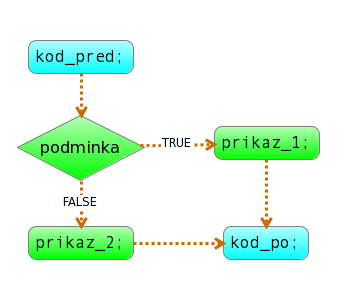
\includegraphics[height=35mm]{img/if.png}
	\column{6cm}
		\begin{verbatim}
		if (podminka) { prikaz_1; }
		else { prikaz_2; }
		\end{verbatim}
	\end{columns}
\end{frame}

\begin{frame}[fragile]
	\frametitle{\texttt{if}}
	\begin{columns}
	\column{50mm}
		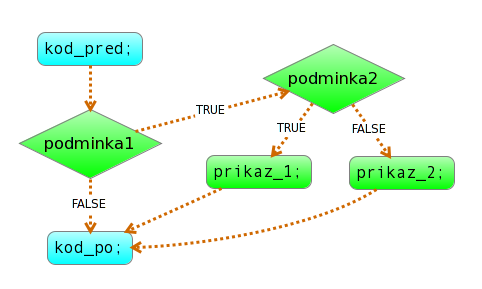
\includegraphics[width=50mm]{img/if_if.png}
	\column{6cm}
		\begin{verbatim}
		if (podminka1)
		if (podminka2) { prikaz_1; }
		else { prikaz_2; }
		\end{verbatim}
	\end{columns}
\end{frame}

\begin{frame}[fragile]
	\frametitle{\texttt{switch}}
	\begin{columns}
	\column{50mm}
		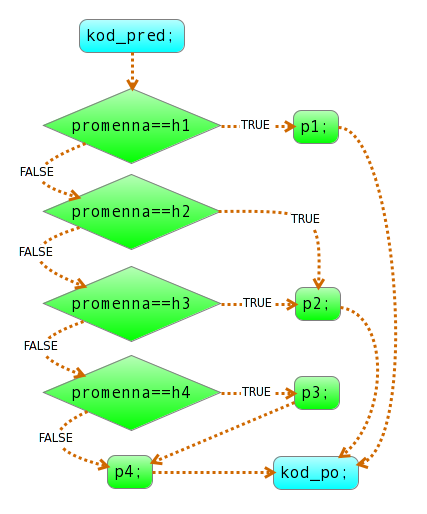
\includegraphics[width=50mm]{img/switch.png}
	\column{6cm}
		\begin{verbatim}
		switch(promenna)
		{
		    case h1: p1; break;
		    case h2:
		    case h3: p2; break;
		    case h4: p3;
		    default: p4; break;
		}
		\end{verbatim}
	\end{columns}
\end{frame}

\begin{frame}[fragile]
	\frametitle{\texttt{for}}
	\begin{columns}
	\column{50mm}
		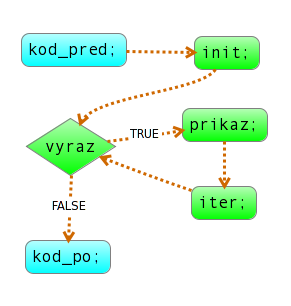
\includegraphics[width=50mm]{img/for.png}
	\column{6cm}
		\begin{verbatim}
		for (init; vyraz; iter)
		{
		    prikaz;
		}
		\end{verbatim}
	\end{columns}
\end{frame}

\begin{frame}[fragile]
	\frametitle{\texttt{while}, \texttt{do}}
	\begin{columns}
	\column{50mm}
		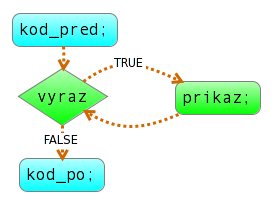
\includegraphics[width=35mm]{img/while.png}\\
		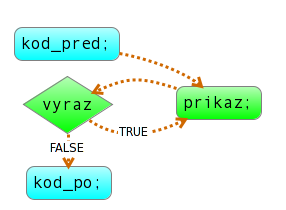
\includegraphics[width=35mm]{img/do.png}
	\column{6cm}
		\begin{verbatim}
		while(vyraz) { prikaz; }

		do { prikaz; } while(vyraz);
		\end{verbatim}
	\end{columns}
\end{frame}

\begin{frame}[fragile]
	\frametitle{\texttt{break}, \texttt{continue}}
	\begin{columns}
	\column{50mm}
		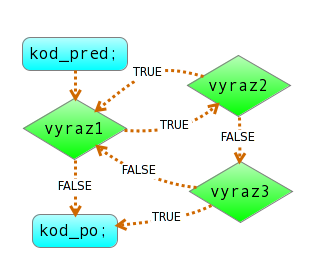
\includegraphics[width=40mm]{img/break.png}
	\column{6cm}
		\begin{verbatim}
		while(vyraz1) 
		{ 
		    if (vyraz2) continue;
		    if (vyraz3) break;
		}
		\end{verbatim}
	\end{columns}
\end{frame}


\section{Práce na cvičení}
\subsection{Procvičení operátorů}

\begin{frame}
	\frametitle{Semafor}
	\begin{itemize}
		\item{implementujte přepínající se semafor}
		\item{v nekonečném cyklu provádějte čekání \texttt{sleep(1);} z \texttt{unistd.h}}
		\item{následované přepnutím a vypsáním stavu semaforu}
		\item{aktuální stav semaforu udržujte}
		\begin{enumerate}
			\item{v samostatných proměnných vhodného typu}
			\item{v jedné celočíselné proměnné jako bitovou masku}
		\end{enumerate}
	\end{itemize}
\end{frame}

\begin{frame}
	\frametitle{Postup práce}
	\begin{itemize}
		\item{u každého příkladu postupjte systematicky}
		\item{vytvořet si projekt}
		\item{nastavte si ho}
		\item{vytvořte si základní kostru main, které nebude nic dělat, ale půjde přeložit a spustit}
		\item{postupně přidávejte funkčnost}
	\end{itemize}
\end{frame}

\subsection{Standardní obsah cvičení}

\begin{frame}
	\frametitle{Práce na cvičení}
	\begin{itemize}
		\item{\href{http://elearning.simontoth.cz/public/pb071\_cviceni}{http://elearning.simontoth.cz/public/pb071\_cviceni}}
	\end{itemize}
\end{frame}

\section{Konec}
\subsection{Konec}

\begin{frame}
	\frametitle{To je pro dnes vše...}
\end{frame}

\section{Kontaktní informace}
	\subsection{Pracovní}

\begin{frame}[label=kontakt-simontoth]
	\frametitle{Mgr. Šimon Tóth}
	\begin{itemize}
		\item{Gotex (Šumavská 15) - kanceláře Cesnet (B310)}
	\end{itemize}
	
	\begin{center}
	\begin{columns}

	\column{0.48\textwidth}
		\begin{itemize}
			\item{Ph.D. student / externí lektor}
			\item{Fakulta informatiky MU}
			\item{toth@fi.muni.cz}
			\item{tel. 549 49 6446}
		\end{itemize}

	\column{0.48\textwidth}
		\begin{itemize}
			\item{Výzkumný pracovník}
			\item{Cesnet z.s.p.o.}
			\item{simon@cesnet.cz}
			\item{tel. 234 680 235}
		\end{itemize}

	\end{columns}
	\end{center}

\end{frame}

	\subsection{Osobní}

\begin{frame}
	\frametitle{Mgr. Šimon Tóth}
		Osobní
		\begin{itemize}
			\item{kontakt@simontoth.cz}
			\item{tel. 776 565 424}
		\end{itemize}
\end{frame}




\end{document}
